\begin{center} 
\emph{``Your sacred space is where you can find yourself again and again.'' -- Joseph Campbell}
\end{center}

\section{Vector Spaces}\label{sec:vector}

Now that we have learned about fields and linear equations, the next important linear structure should discuss is that of \emph{linear combination}. In order to define this, we first need a notion of a vector. We say that a mathematical quantity is a \emph{vector} if we can add two vectors together to create a third vector and we can scale a vector by a scalar (hence the name). Vectors are distinct from scalars. While a scalar is a number, a vector is more complicated than just a number. To distinguish the extra complexity of vectors, vector quantities are denoted either in boldface font, such as $\bb u, \bb v$, or with an arrowhead above the symbol, such as $\vec u, \vec v$. The following definition makes precise this notion.\\

\begin{Def}\label{def:vectorspace} A \textbf{vector space} over a field $F$ is a nonempty set $V$ of elements, called \textbf{vectors}, on which are defined two operations, called \textbf{addition} $+ : V\times V \to V$ and \textbf{scalar multiplication} $\cdot : F\times V \to V$, such that for all $\bb u, \bb v, \bb w \in V$ and all scalars $c, d\in F$, the following eight axioms hold:
\setlength{\columnsep}{30pt}
\begin{multicols}{2}
\begin{enumerate}[!DEF!, start=1]
\item\label{item:vsaddassoc} \textbf{Additive Associativity}: $\bb u + \bb v = \bb v + \bb u$ 
\item\label{item:vsaddcomm} \textbf{Additive Commutativity}:\\ \mbox{}\hfill$(\bb u + \bb v) + \bb w = \bb u + (\bb v +  \bb w)$ 
\item\label{item:vsaddident} \textbf{Additive Identity}: There exists  a vector $\bb 0\in V$, such that $\bb u + \bb 0 = \bb 0 + \bb u = \bb u$ 
\item\label{item:vsaddinv} \textbf{Additive Inverse}: For each $\bb u$, there exists a vector $-\bb u\in V$, such that\\ \mbox{}\hfill$\bb u + (-\bb u) = (-\bb u) + \bb u = \bb 0$ \columnbreak
\item\label{item:vsleftdist} \textbf{Left Distributivity}: $c(\bb u + \bb v) = c\bb u + c\bb v$ 
\item\label{item:vsrightdist} \textbf{Right Distributivity}: $(c+d)\bb u = c\bb u + d\bb u$
\item\label{item:vsmultassoc} \textbf{Multiplicative Associativity}:\\ \mbox{}\hfill$c(d\bb u) = (cd)\bb u$ 
\item\label{item:vsmultiden} \textbf{Multiplicative Identity}: $1\bb u = \bb u$\\\\
\end{enumerate}
\end{multicols}
\end{Def}

\begin{Exam}\begin{multicols}{2}
In physics, a vector represents a mathematical quantity with both magnitude and direction, such as a force applied to an object. Vectors are thus represented as arrows pointing in the given direction and whose length represents the magnitude of the vector. Physical vectors are also free to move about in space, that is, this exact location does not matter so long as their length nor direction does not change. Therefore, the\columnbreak

\mbox{}
\begin{center}
\begin{tikzpicture}
\draw[-latex, ultra thick] (0,0) -- (1,1) node[midway, below right] {$\bb v$};
\draw[-latex, ultra thick, blue] (3,2) -- (4,3) node[midway, below right] {$\bb v$};
\draw[-latex, ultra thick, red] (-1,2) -- (0,3) node[midway, below right] {$\bb v$};
\end{tikzpicture}
\end{center}
\end{multicols}
\vspace{-10 pt} \noindent
 three arrows illustrated above represent that same vector $\bb v$. Hence, the arrow is determined by the relative displacement of the head of the arrow from its tails. These vectors can be added together by the so-called \emph{parallelogram rule}: begin by placing the tails of the two vectors $\bb u$ and $\bb v$ together, form a parallelogram whose parallel sides correspond to $\bb u$ with a copy of $\bb u$ and $\bb v$ with a copy of $\bb v$; the sum $\bb u + \bb v$ is the unique vector which is the diagonal of the parallelogram whose tail agrees with the tail of $\bb u$ and $\bb v$, as displayed:

\begin{multicols}{3}
\begin{center}
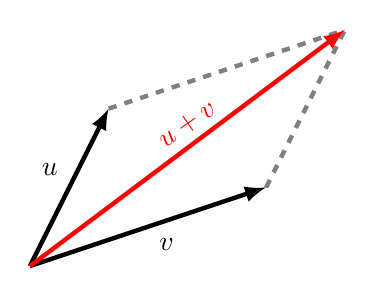
\begin{tikzpicture}
\draw[dashed, ultra thick, gray] (1,2) -- (4,3);
\draw[dashed, ultra thick, gray] (3,1) -- (4,3);
\draw[-latex, ultra thick] (0,0) -- (3,1) node[midway, below right] {$\bb v$};
\draw[-latex, ultra thick] (0,0) -- (1,2) node[midway, above left] {$\bb u$};
\draw[-latex, ultra thick, red] (0,0) -- (4,3) node[midway, above, yshift = -5] {\rotatebox{35}{$\bb u + \bb v$}};
%\path(2,-1) node[below] {The Parallelogram Rule};
\end{tikzpicture}
\vfill \textbf{The Parallelogram Rule}
\end{center}

\begin{center}
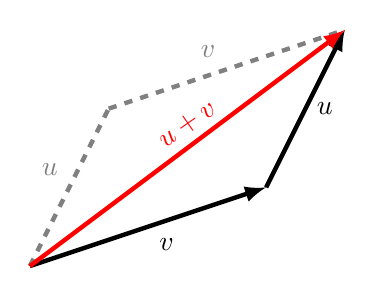
\begin{tikzpicture}
\draw[dashed, ultra thick, gray] (1,2) -- (4,3) node[above left, midway] {$\bb v$};
\draw[dashed, ultra thick, gray] (0,0) -- (1,2) node[above left, midway] {$\bb u$};
\draw[-latex, ultra thick] (0,0) -- (3,1) node[midway, below right] {$\bb v$};
\draw[-latex, ultra thick] (3,1) -- (4,3) node[midway, right] {$\bb u$};
\draw[-latex, ultra thick, red] (0,0) -- (4,3) node[midway, above, yshift = -5] {\rotatebox{35}{$\bb u + \bb v$}};
\end{tikzpicture}
\vfill $\bb u + \bb v = \bb v + \bb u$
\end{center}

\begin{center}
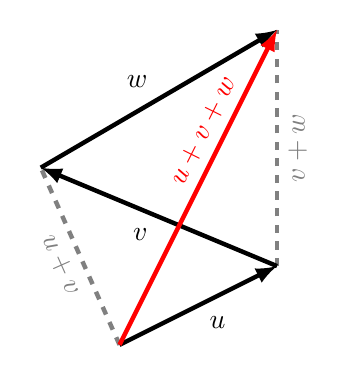
\begin{tikzpicture}
\draw[, ultra thick, dashed, gray] (0,0) -- (-1,2.25) node[midway, below, sloped] {$\bb u+\bb v$};
\draw[, ultra thick, dashed, gray] (2,1) -- (2,4) node[midway, below, sloped] {$\bb v+\bb w$};
\draw[-latex, ultra thick] (0,0) -- (2,1) node[midway, below right] {$\bb u$};
\draw[-latex, ultra thick] (2,1) -- (-1,2.25) node[midway, below left] {$\bb v$};
\draw[-latex, ultra thick] (-1,2.25) -- (2,4) node[midway, above left] {$\bb w$};
\draw[-latex, ultra thick, red] (0,0) -- (2,4) node[pos=0.65, sloped, above] {$\bb u + \bb v + \bb w$};
\end{tikzpicture}
\end{center}
\vfill $(\bb u + \bb v) + \bb w = \bb u + (\bb v + \bb w)$
\end{multicols}
The second diagram shows why arrow addition is commutative, as the two paths from the tail of $\bb u+\bb v$ to head produce the same vector. In particular, the black, solid path comprises $\bb v+\bb u$ while the gray, dashed path comprises $\bb u+\bb v$, and both paths have the same starting and ending points. The third diagram likewise demonstrates how three or more vectors are added together and why arrow addition is associative, as the path following $(\bb u + \bb v)$ then $\bb w$ produces the same vector as the path following $\bb u$ then $(\bb v+\bb w$).

The zero vector $\bb 0$ would be simply a point in space, that is, the vector with no magnitude nor direction. Notice that adjoining a point to the head or tail will neither lengthen the arrow nor turn it. Thus, $\bb v+\bb 0 =\bb v$. Additionally, given a vector $\bb v$, $-\bb v$ is defined as the arrow with the same length but pointing in the opposite direction. It holds that $\bb v + (-\bb v) = (-\bb v) + \bb v = \bb 0$.
\begin{center}
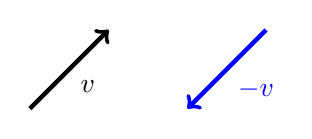
\begin{tikzpicture}
\draw[->, ultra thick] (0,0) -- (1,1) node[midway, below right] {$\bb v$};
\draw[->, ultra thick, blue] (3,1) -- (2,0) node[midway, below right] {$-\bb v$};
\end{tikzpicture}
\end{center}

\noindent We define scalar multiplication of arrows by multiplying the length of the arrow by the scalar (and switching directions if the scalar is negative). Clearly, $1\bb v=\bb v$, since the length of the arrow is unchanged, and $c(d\bb u) = (cd)\bb u$, since stretching a vector by a factor of $d$ then stretching by a factor of $c$ as the net affect of stretching the arrow by a factor of $cd$. It is left as an exercise of the reader to prove that two distributive laws. Therefore, the set of arrow in space forms a vector space under these operations.
\end{Exam}\vs

\begin{Exam}
Another type of vector is an array of numbers. Let $F$ be a field. Then a \textbf{column vector} is an array of $n$ scalars from $F$ such that the array is oriented vertically, e.g. $\bb v = \vr{1\\2\\3}$. A \textbf{row vector} likewise is an array of $n$ scalars such that the array is oriented horizontally, e.g.  $\bb v =(1, 2, 3)$. Our notation of a row vector agrees with the commonly used  notation  for coordinates of points in Cartesian geometry. As such, we naturally identify these arrays of scalars with points in space. The difference between row vectors and column vectors is purely notational, and we will use the two notations interchangeably.\footnotemark[2]  The order of the scalars in the array does matter, e.g. $(1, 2, 3) \neq (2,3, 1)$.\\

Let $F^n$ denote the set of all column vectors with $n$ entries coming from the field $F$, for example, for example, \[\mtx{c}{\pi\\ 0\\ -\sqrt{17}} \in \R^3,\quad \vr{1-2i \\  \frac{1}{2}-\frac{5}{2}i}\in \C^2,\quad \text{ or }\quad \vr{1\\2\\0\\2\\1}\in \Z_3^5.\footnotemark[8]\]

Addition of column vectors is component-wise, that is, scalars in the corresponding positions are added together:
\begin{equation} \bb u+ \bb v = \mtx{c}{u_1\\u_2\\\vdots\\u_n} + \mtx{c}{v_1\\v_2\\\vdots\\v_n} = \mtx{c}{u_1+v_1\\u_2+v_2\\\vdots\\u_n+v_n}. \end{equation}  For scalar multiplication, every component is multiplied by the scalar, that is:
\begin{equation} c\bb x = c\mtx{c}{x_1\\x_2\\\vdots\\x_n}= \mtx{c}{cx_1\\cx_2\\\vdots\\cx_n}. \end{equation}   Here the zero vector $\bb 0$ is the array of all zeros and $-\bb v=(-1)\bb v$. We show that this definition of vector addition satisfies the additive associativity axiom:
\begin{multline*}\bb u+(\bb v+\bb w) = \mtx{c}{u_1\\u_2\\\vdots\\u_n} + \left(\mtx{c}{v_1\\v_2\\\vdots\\v_n} + \mtx{c}{w_1\\w_2\\\vdots\\w_n}\right) = \mtx{c}{u_1\\u_2\\\vdots\\u_n} + \mtx{c}{v_1+w_1\\v_2+w_2\\\vdots\\v_n+w_n} = \mtx{c}{u_1+(v_1+w_1)\\u_2+(v_2+w_2)\\\vdots\\u_n+(v_n+w_n)}\\ \overset{(*)}{=} \mtx{c}{(u_1+v_1)+w_1\\(u_2+v_2)+w_2\\\vdots\\(u_n+v_n)+w_n)} = \mtx{c}{u_1+v_1\\u_2+v_2\\\vdots\\u_n+v_n} + \mtx{c}{w_1\\w_2\\\vdots\\w_n} = \left(\mtx{c}{u_1\\u_2\\\vdots\\u_n} + \mtx{c}{v_1\\v_2\\\vdots\\v_n}\right) + \mtx{c}{w_1\\w_2\\\vdots\\w_n} = (\bb u + \bb v) + \bb w,
\end{multline*} where the marked equality $(*)$ follows from the additive associtivity of the field $F$. The remaining axioms of a vector space are left as an exercise to the reader. Therefore, $F^n$ is a vector space, the one we will place the most focus on in this text.
\end{Exam}\vs

\begin{Exam} Let $\bb u = \vr{ 6\\-2\\ 2}, \bb v = \vr{ -3\\0\\ 5} \in \R^3$. Then 
\[\bb u + \bb v = \vr{ 6\\-2\\ 2} + \vr{ -3\\0\\ 5} = \vr{ 6-3\\ -2+0\\ 2+5} = \vr{ 3\\ -2\\ 7}.\]
 If $\bb v = \vr{-1\\ 3\\2}\in \R^3$, then 
\[3\bb v = 3\vr{-1\\ 3\\2} = \vr{ -3\\ 9\\6}. \qedhere\]
\end{Exam}\vs

\begin{Def}\label{def:linearcombo} Given vectors $\bb v_1, \bb v_2, \ldots, \bb v_n\in F^m$ and scalars $c_1, c_2, \ldots, c_n\in F$, the vector $\bb x$ given as 
\[\bb x = c_1\bb v_1 + c_2\bb v_2 + \ldots + c_n\bb v_n\] is called a \textbf{linear combination} of $\bb v_1, \bb v_2, \ldots, \bb v_n$ with \textbf{coefficients} $c_1, c_2, \ldots, c_n$. \\
\end{Def}\vs

A linear combination is a way of combining vectors using addition and scalar multiplication. These vectors operations, of course, depend entirely on the field of scalars.\\

\begin{Exam} Let us simplify the following linear combinations over the vector spaces $\C^2$ and $\Z_3^3$, respectively.
\begin{enumerate}
\item $2\mtx{c}{3\\ i} + i\mtx{c}{2+i\\ 3+5i} = \mtx{c}{6\\2i} + \mtx{c}{-1+2i\\ -5+3i} = \mtx{c}{6+(-1+2i)\\ 2i + (-5+3i)} = \mtx{c}{5+2i\\-5+5i}$.\\

\item $\vr{0\\1\\2} + 2\vr{1\\1\\1} + 2\vr{1\\0\\2} \equiv \vr{0\\1\\2} + \vr{2\\2\\2} + \vr{2\\0\\1} \equiv \mtx{c}{0+2+2\\ 1+2+0\\2+2+1} \equiv \mtx{c}{4\\3\\5} \equiv \mtx{c}{1\\0\\2} \pmod 3. \hfill\qedhere$
\end{enumerate}
\end{Exam}\vs

Vectors can also be many other things, like matrices,  functions, sequences of numbers. Even linear equations can be vectors. \\

\begin{Exam}\label{exam:vectorspaceproof} Let $V$ be the set of linear equations with $n$ variables, say $x_1, x_2,\ldots, x_n$ with coefficients coming from the field $F$.  For example, 
\[c_1x_1+\ldots + c_nx_n = b_1\] is an element of $V$ for $c_1,\ldots, c_n, b_1\in F$. Likewise, if \[d_1x_1+\ldots + d_nx_n=b_2\] is another linear equation in $V$, then 
\[\begin{alignedat}{100}
&& (c_1x_1\ &+\ & \ldots\ & +\ & c_nx_n\ & =\ & b_1) \\
+\ && (d_1x_1\ &+\ &\ldots\ & +\ & d_nx_n\ &=\ &b_2)\\ \hline
&&(c_1+d_1)x_1\ &+\ & \ldots\ & +\ & (c_n+d_n)x_n\ & =\ & (b_1+b_2)
\end{alignedat}\] Note that $c_i+d_i, b_1+b_2\in F$ for all $i$. Thus, the sum of equations is a member of $V$, that is, it is a vector too. Similarly, if $a\in F$, then $c_1x_1+\ldots + c_nx_n = b_1$ scaled by $a$ is the linear equation 
 \[(ac_1)x_1+\ldots + (ac_n)x_n = (ab_1).\] As $ac_i, ab_1\in F$ for all $i$, this equation is likewise a vector. Therefore, $V$ is a vector space. Let $E_1, E_2, \ldots, E_m \in V$ be a list of linear equations with common solution $\bb x \in F^n$. Then $\bb x$ is a solution to any linear combination $a_1E_1 + a_2E_2 +\ldots + a_mE_m$. 
\end{Exam}\vs

\begin{Thm}\label{thm:vectorprop} The following properties hold for any $F$-vector space $V$. Let $\bb u \in V$ and $c\in F$.
\begin{enumerate}[!THM!, start=1]
\begin{multicols}{2}
\item\label{item:vectorpropuniquezero} The zero vector $\bb 0$ in $V$ is unique.\\
\item\label{item:vectorpropuniqueinverse} The additive inverse of $\bb u$ is unique.\\
\end{multicols}
\begin{multicols}{3}
\item\label{item:vectorpropzeroscalar} $0\bb u = \bb 0$.\\
\item\label{thm:vectorpropzerovector} $c\bb 0 = \bb 0$.\columnbreak
\item\label{thm:vectorpropnegscalar} $-\bb u = (-1)\bb u$.
\end{multicols}
\end{enumerate}
\end{Thm}
\begin{proof}
\begin{enumerate}[!DEF!,start=1]
\item Suppose there is a vector $\bb\theta \in V$ such that $\bb\theta + \bb v = \bb v + \bb\theta = \bb v$ for all $\bb v\in V$. Then 
\[\bb 0 = \bb 0 + \bb \theta = \bb \theta.\] Therefore, $\bb 0$ is the unique vector with this property.\\

\item Like the last property, suppose that $\bb u' \in V$ has the property that $\bb u + \bb u' = \bb u' + \bb u = \bb 0$. Then
\[\bb u' = \bb u' + \bb 0 = \bb u' + (\bb u + -\bb u) = (\bb u' + \bb u) + -\bb u = \bb 0 + -\bb u = -\bb u.\] Therefore, $-\bb u$ is the unique vector with this property.\\

\item First, \[0\bb u = (0+0)\bb u = 0\bb u + 0\bb u.\] Adding $-0\bb u$ to both sides of the equation gives $\bb 0 = 0\bb u$.\\

The remaining parts are left as exercises to the reader.\hfill$\qedhere$
%\item Now, 
%\[\bb 0 = 0\bb 0 = (c0)\bb 0  = c(0\bb 0) = c\bb0.\]
%
%\item Finally, 
%\[\bb u + (-1)\bb u = 1\bb u + (-1)\bb u = (1-1)\bb u = 0\bb u = \bb 0.\] Therefore, $(-1)\bb u = -\bb u$. \hfill$\qedhere$
\end{enumerate}
\end{proof}

%%%%%%%%%%%%%%%%%%% Exercises %%%%%%%%%%%%%%%%%%%
\startExercises{vector}

\noindent For Exercises \ref{true:vsstart}-\ref{true:vsstop}, determine with the statement is true or false. If false, correct the statement so that it is true.
\begin{enumerate}[!HW!, start=1]
\item\label{true:vsstart}\label{true:vsstop} For any \hyperref[def:vectorspace]{vector space} $V$, $\emptyset\in V$. %Da Huo
\end{enumerate}

\noindent For Exercises \ref{exer:linearcomborealstart}-\ref{exer:linearcomborealstop}, simplify the \hyperref[def:linearcombo]{linear combination}. 
\begin{enumerate}[!HW!]
\begin{multicols}{2}
\item\label{exer:linearcomborealstart} $5\vr{1\\2\\4}+3\vr{0\\2\\1}+4\vr{1\\1\\1}$ %Cameron Dix
\itemspade $3\vr{-1\\0\\1} + 2\vr{0\\0\\1}-2\vr{3\\4\\0}$
\end{multicols}
\begin{multicols}{2}
\item $\vr{3\\2\\1} + \mtx{c}{5\\8\\10} + \vr{0\\0\\5}$ %Sherie Ayag
\item $-1\vr{3\\0\\1}+\vr{1\\2\\4} + 3\vr{2\\4\\1}$ %Jacob Newey
\end{multicols}
\begin{multicols}{2}
\item $7\vr{3\\0\\2}+2\vr{8\\-3\\5}-3\vr{-2\\-2\\0}$ %Grayson Walker
\item $8\vr{1\\4\\3} +2\vr{5\\0\\4} -4\vr{1\\0\\1}$ %Yinglong Niu
\end{multicols}
\begin{multicols}{2}
\item $(2+5i)\vr{3\\4} - (3-2i)\mtx{c}{7+i\\6+2i}$ %Heming Zu
\itemspade $(3+2i)\vr{1\\2} -(1-2i)\mtx{c}{3+4i \\ 1+i}$
\end{multicols}
\begin{multicols}{2}
\item $(2+i)\mtx{c}{1+i\\i} + \mtx{c}{2i\\1+2i}$ %Cameron Dix
\item $(2+4i)\vr{2\\3} - (3-2i)\mtx{c}{1+2i\\2-i}$ %Jaimie Goldberg 
\end{multicols}
\begin{multicols}{2}
\item $(1+i)\mtx{c}{1-i\\2+i}-(1-i)\mtx{c}{3+i\\4-i}$ %Yinglong Niu
\item $(1-i)\mtx{r}{1\\2\\-1} + \vr{2\\3\\5} -(2+3i)\vr{1\\4\\2}$ %Jacob Newey
\end{multicols}
\begin{multicols}{2}
\item $(4+5i)\vr{3\\5\\2} +(3-2i)\vr{1+3i\\2-3i\\2+5i}$ %Kyle Wood
\item $2\vr{2\\1} - \vr{1\\0} +2\vr{1\\1} \pmod3$ %Jacob Newey
\end{multicols}
\begin{multicols}{2}
\item $-10\vr{3\\2}+\vr{5\\6} \pmod7$ %Cameron Dix
\itemspade $\vr{1\\0\\1} + \vr{1\\1\\0} + \vr{1\\1\\1} \pmod 2$
\end{multicols}
\begin{multicols}{2}
\item $6\vr{1\\3\\4} + 2\vr{1\\1\\5} + \vr{1\\1\\1} \pmod 3$ %Kaylee Hall
\item $\vr{3\\4\\3}+\vr{4\\1\\1}+\vr{0\\1\\1} \pmod5$ %Cameron Dix
\end{multicols} \pagebreak
\begin{multicols}{2}
\item $2\vr{1\\2\\3}+3\vr{3\\2\\1}+4\vr{0\\1\\0}\pmod5$ %anon
\itemspade $4\vr{1\\0\\0\\2} + 2\vr{2\\3\\1\\0} + \vr{1\\2\\3\\4}\pmod5$
\end{multicols}
\begin{multicols}{2}
\item $3\vr{-1\\2\\-3\\0}-2\vr{1\\2\\2\\1}+\vr{2\\3\\0\\1}\pmod5$ %Jacob Newey

\item \label{exer:linearcomborealstop} $\vr{4\\2\\3\\1} + 2\vr{0\\1\\4\\3} + 3\vr{1\\1\\2\\3}\pmod5$\ %Hailey Checketts
\end{multicols}
\end{enumerate}

\begin{enumerate}[!HW!]
\itemspade Prove parts \ref{thm:vectorpropzerovector} and \ref{thm:vectorpropnegscalar} of \thmref{thm:vectorprop}.
\end{enumerate}
\begin{enumerate}[!HW!, label=$\spadesuit$ \arabic*., ref=\arabic*]
\item\label{exer:polynomialspace} Let $\P_n =\{a_0 + a_1x + a_2x^2 + \ldots + a_nx^n \mid a_0, a_1, a_2,\ldots, a_n\in F\}$ be the set of polynomials of degree at most $n$ and coefficients from a \hyperref[def:field]{field} $F$. Show that $\P_n$ is a \hyperref[def:vectorspace]{vector space}, hence we may view polynomials as vector quantities. (More specifically, show that the sum of two polynomials is again a polynomial and the scalar multiple of a polynomial is likewise a polynomial, similar to the method introduced in Example \ref{exam:vectorspaceproof}).
\end{enumerate}

\noindent Note that the way we defined vector addition and scalar multiplication over \hyperref[note:Fn]{$F^n$} is essentially the only way to do it to guarantee the \hyperref[def:vectorspace]{vector space axioms}. For Exercises \ref{exer:vsNewScalarsstart}-\ref{exer:vsNewScalarsstop}, we will redefine scalar multiplication over $F^3$ (and keep vector addition the same). Find a counterexample for why this alternative definition of scalar multiplication fails at least one \hyperref[def:vectorspace]{vector space axiom} or property and hence does not produce a genuine vector space. Answers may vary.
\begin{enumerate}[!HW!, label=$\spadesuit$ \arabic*., ref=\arabic*]
\begin{multicols}{2}
\item\label{exer:vsNewScalarsstart} Redefine scaling: $c\vr{x_1\\x_2\\x_3} = \vr{x_1\\x_2\\x_3}$
\item Redefine scaling: $c\vr{x_1\\x_2\\x_3} = \mtx{c}{cx_1\\x_2\\x_3}$
\end{multicols}
\begin{multicols}{2}
\item Redefine scaling: $c\vr{x_1\\x_2\\x_3} = \vr{-cx_1\\-cx_2\\-cx_3}$
\item\label{exer:vsNewScalarsstop} Redefine scaling: $c\vr{x_1\\x_2\\x_3} = \mtx{c}{0\\cx_2\\cx_3}$
\end{multicols}
\end{enumerate}

\pagebreak
%%%%%%%%%%%%%%%%%%% Footnotes %%%%%%%%%%%%%%%%%%%
\mbox{}\vfill

\footnotetext[2]{From a vector perspective, the notion of a column vector $\vr{1\\2\\3}$, a row vector $[1\ 2\ 3]$, and a geometric point $(1,2,3)$ are all the same. Why have different notations then? In other contexts, it is helpful to distinguish between them. In calculus or physics, a distinction between points and vectors (aka arrows) is sometimes desired (although often unnecessary). Thus, points have their usual notation and arrows are given a different notation, which may include the column or row vector notation we have already introduced or some other notation that we will not use here, e.g. $\langle 1, 2, 3\rangle$. As arrows can be moved anywhere in space without changing their value, the vectors are often placed in \emph{standard position}, meaning its tail is on the origin. Then the head of the arrow is a unique point in space which characterizes this arrow. This standard representation of the vector, sometimes called its \emph{algebraic form}, is very desirable as the algebraic computations are far simpler their their geometric counterparts. For this reason, we see not strong reason to distinguish between arrows in space and the coordinates that they are pointing at. The only perspective that we will distinguish between a column vector and a row vector herein is when we consider them matrices, such as in \chapref{3rd}. This may be imperative for matrix operations, such as multiplication. Under the matrix perspective, a column vector is just an $n\times 1$ matrix, and a row vector is just a $1\times n$ matrix.}

%Andrew Biskey
\footnotetext[8]{The combined notations of the set $\Z_p$, which is a field whose subscript defines the modulus, and the vector space $F^n$, whose superscripts defines the number of entries in each vector, conveys information about the vector space $\Z_p^n$.  For example, $\Z_3^5$ denotes the vector space whose vectors comprise of five elements in the array that are integers congruent modulo 3, e.g, $\vr{1\\2\\0\\2\\1}$. Note that no integer in $\Z_3^n$ ever needs to be greater that $2$ or smaller than $0$, as all those integers are reducible modulo $3$. Hence, $\Z_3^5$ contains exactly $3^5=243$ distinct vectors. In general, the vector space $\Z_p^n$ will contain exactly $p^n$ many vectors.}
\pagebreak